% The bundled cycle: why the margin of the equality locus vanishes.  Three
% panels -- the graph at (6,3) with arc sizes (2,2,1,1), the leverage in closed
% form with the instances it is checked at, and the rank-two drop plane -- and a
% footer carrying the gap identity.  There is no projection; x = y = 1cm.
%
% LAYOUT.
%   left, the graph        x -0.52 .. 4.20  square of side 2.20 with corners
%                          v_0 = (0.75,-0.75), v_1 = (2.95,-0.75),
%                          v_2 = (2.95,-2.95), v_3 = (0.75,-2.95); arc j runs
%                          from v_j to v_{j+1}, and v_3 is the ground.  The
%                          arc-size tag on the left edge overhangs the square,
%                          which is what puts the panel's left edge at -0.52
%   middle, the leverage   x 4.55 .. 9.85   three formula lines at -0.20, -0.56
%                          and -0.92, a head at -1.46 and seven rows at
%                          -1.90 - 0.32r, r = 0..6, in columns at 4.60, 5.60
%                          and 7.35, then one note at -4.42
%   right, the drop plane  x 10.30 .. 15.40 box [-2.4,2.4]^2 in the drops, at
%                          0.85cm a unit, centred at (12.85,-2.42)
%   footer                 five lines at -5.30, -5.66, -6.02, -6.38, -6.74,
%                          from x = 0; the widest of the five is 14.94cm
% Panel titles sit at y = 0.20.  The plate runs from -0.52, the arc-size tag on
% the left edge of the square, to 15.32, the $d_1$ label of the drop plane, so
% 15.84cm wide, inside the 16.20cm text block.
%
% THE FAMILY.  Take the (k+1)-cycle, replace arc j by a bundle of p_j >= 1
% parallel edges, and write n = sum_j p_j.  Put the uniform design weight 1/n on
% the n edges and the conductance 1/(p_j (n - p_j)) on every edge of bundle j.
% Then every transversal -- one edge out of each of k of the k+1 bundles --
% dominates, and no k-subset dominates strictly.
%
% THE DRAWN INSTANCE, exactly.  k = 3, arc sizes p = (2,2,1,1), n = 6, so the
% design is at (6,3):
%   t_e = 1/6 at all six edges
%   conductance 1/(2 x 4) = 1/8 on the four edges of arcs 0 and 1,
%               1/(1 x 5) = 1/5 on the single edges of arcs 2 and 3
%   ell_e = ((k-1)n + p)/(k p) = (12 + p)/(3p), so 7/3 at p = 2 and 13/3 at p = 1
%   P_ee = (k-1)/(kp) + 1/(kn) = 2/(3p) + 1/18, so 7/18 and 13/18
%   sum_e t_e ell_e = 4(7/3)/6 + 2(13/3)/6 = (28/3 + 26/3)/6 = 3 = k
% The closed form was checked against the graph directly: forming the reduced
% Laplacian L = sum_e c_e b_e b_e^T on the coordinates (y_0, y_1, y_2) with the
% ground deleted, the leverage score c_e b_e^T L^{-1} b_e comes out at
% (k-1)/(kp) + 1/(kn) at every one of the seven bundlings listed on the plate,
% and the leverage scores sum to k in each.
%
% THE GAP IDENTITY, with the cancellation named.  Write d_j for the potential
% drop across arc j, so that sum_j d_j = 0 around the cycle.  A transversal
% omitting arc j_0 selects one edge of each other arc, and the selected form
% carries n c_e d_j^2 = n d_j^2/(p_j(n - p_j)) at each j =/= j_0, while the full
% form carries d_j^2/(n - p_j) at every j -- the bundle of size p_j contributing
% p_j copies of c_e = 1/(p_j(n-p_j)).  Subtracting term by term, at j =/= j_0
%   n/(p_j(n-p_j)) - 1/(n-p_j) = (n - p_j)/(p_j(n-p_j)) = 1/p_j,
% and the only term of the full form with no partner is the one at j_0, which
% survives as -d_{j_0}^2/(n - p_{j_0}).  Now d_{j_0} = -sum_{j =/= j_0} d_j and
% n - p_{j_0} = sum_{j =/= j_0} p_j, so that surviving term is exactly the
% subtracted square, and the gap is
%   sum_{j =/= j_0} d_j^2/p_j - (sum_{j =/= j_0} d_j)^2 / sum_{j =/= j_0} p_j,
% Engel's form of Cauchy-Schwarz: nonnegative always, zero exactly on the ray
% d_j proportional to p_j over j != j_0 -- the dropped coordinate is pinned by
% sum_j d_j = 0 at d_{j_0} = -lambda (n - p_{j_0}), so it never joins the ray.
% That ray is realized by a potential, so the margin is
% zero and not merely small.
%
% THE RANK-TWO PANEL, exactly.  At k = 2 a transversal spans two arcs and the
% two-term deficiency is an exact rational square,
%   d_1^2/p_1 + d_2^2/p_2 - (d_1+d_2)^2/(p_1+p_2)
%     = (d_1 p_2 - d_2 p_1)^2 / (p_1 p_2 (p_1 + p_2)).
% Drawn at (p_1,p_2) = (4,3), a transversal of the (9,2) bundling with arc sizes
% (4,3,2), the gap is (3 d_1 - 4 d_2)^2/84.  The drop plane is the square
% [-2.4,2.4]^2 at 0.85cm a unit, so a drop pair (d_1,d_2) sits at
% (0.85 d_1, 0.85 d_2) from the panel centre (12.85,-2.42).  Three level lines
% are drawn:
%   3 d_1 - 4 d_2 = 0, the tight ray d proportional to (4,3), gap 0, from
%     (-2.4,-1.8) to (2.4,1.8), that is (-2.04,-1.53) to (2.04,1.53);
%   3 d_1 - 4 d_2 = 6, gap 36/84 = 3/7, entering at (-1.2,-2.4) and leaving at
%     (2.4,0.3), that is (-1.02,-2.04) to (2.04,0.255);
%   3 d_1 - 4 d_2 = -6, gap 3/7, from (1.2,2.4) to (-2.4,-0.3), that is
%     (1.02,2.04) to (-2.04,-0.255).
% The two dashed lines bound the region where the margin is below 3/7; between
% them the gap is smaller, and it reaches zero only on the ray.  The two tags
% sit on their own lines: (1.30, 0.975) is on the tight ray, since
% 0.975 = 0.75 x 1.30, and (-1.30, 0.300) is on the line 3 d_1 - 4 d_2 = -6,
% since that line reads y = (3x + 6 x 0.85)/4 in cm and 3(-1.30) + 5.10 = 1.20,
% a quarter of which is 0.300.
%
% THE INSTANCE TABLE.
%   (6,3) (3,1,1,1)  5/3, 13/3        (7,3) (3,2,1,1)  17/9, 8/3, 5
%   (6,3) (2,2,1,1)  7/3, 13/3        (7,3) (2,2,2,1)  8/3, 5
%   (7,3) (4,1,1,1)  3/2, 5           (9,2) (7,1,1)    8/7, 5
%                                     (9,2) (4,3,2)    13/8, 2, 11/4
% All seven tables were reproduced here in exact rational arithmetic from the
% Laplacian of the graph, independently of the closed form: form
% L = sum_e c_e b_e b_e^T on the coordinates with the ground deleted, read
% s_e = c_e b_e^T L^{-1} b_e, and divide by the uniform weight 1/n.
%
% DISCLOSED, on what the kernel evaluates and what it does not.  Each of the
% seven bundlings is an exact tie in the kernel.  Every distinct leverage in the
% five rank-three rows is evaluated there as well.  At rank two what the kernel
% evaluates is not the leverage but its companion, the projection diagonal
% 1/(2n) + 1/(2p): that is 1/18 + 1/14 = 8/63 and 1/18 + 1/2 = 5/9 at (7,1,1),
% and 13/72, 2/9, 11/36 at (4,3,2).  The two rank-two leverage rows on the plate
% are the closed form evaluated here.
%
% DISCLOSED, on scope.  The plate draws one family, not the equality locus: the
% bundled cycles are the cycle matroid U(k,k+1) with parallel extensions, and
% the other rank-three tight class, the diamond, is not among them.  The
% identification of this family with the series-parallel construction of the
% cited literature is an attribution, not a statement proved here or in the
% development.
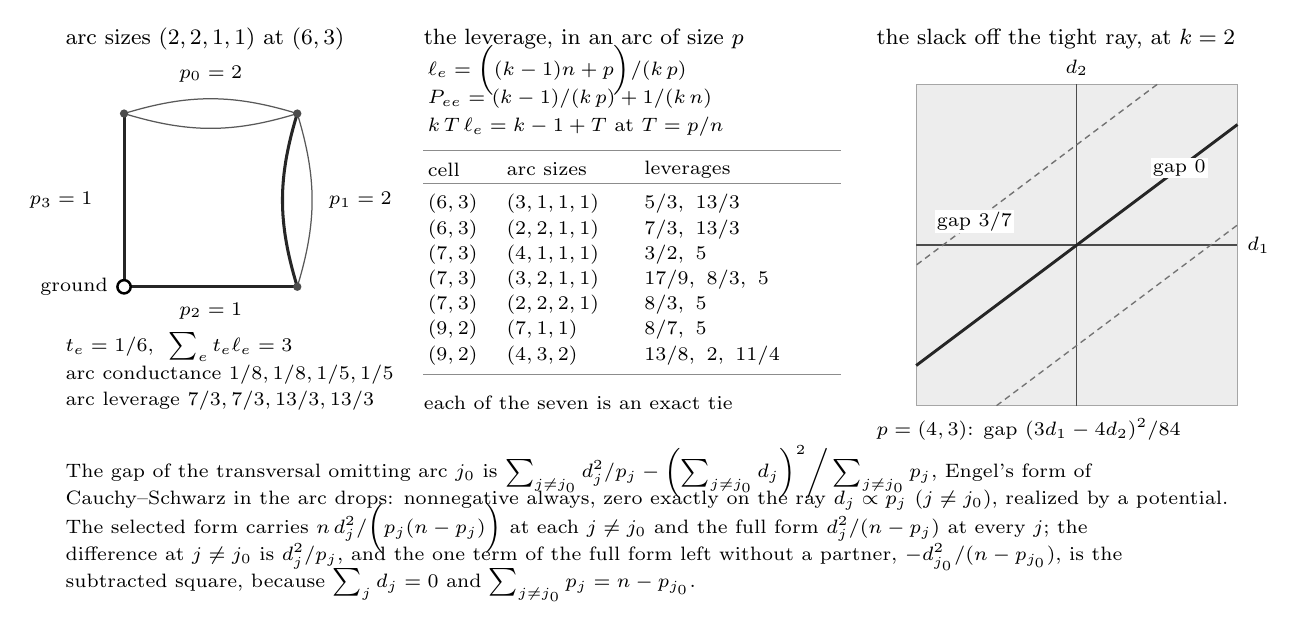
\begin{tikzpicture}[
  x=1cm, y=1cm,
  edge/.style={line width=0.45pt, black!65},
  sel/.style={line width=1.1pt, black!85},
  level/.style={line width=0.5pt, black!55, dashed,
                dash pattern=on 2.2pt off 1.6pt},
  tight/.style={line width=1.05pt, black!85},
  frame/.style={line width=0.3pt, black!35},
  axis/.style={line width=0.4pt, black!70},
  hair/.style={line width=0.25pt, black!45},
  title/.style={font=\footnotesize, anchor=west, inner sep=0pt},
  cell/.style={font=\scriptsize, inner sep=0pt},
  lab/.style={font=\scriptsize, anchor=west, inner sep=0pt},
  tag/.style={font=\scriptsize, fill=white, inner sep=0.7pt},
  note/.style={font=\scriptsize, anchor=west, inner sep=0pt}]

% ===================== left: the bundled 4-cycle ========================
\node[title] at (0.00,0.20) {arc sizes $(2,2,1,1)$ at $(6,3)$};
\coordinate (w0) at (0.75,-0.75);
\coordinate (w1) at (2.95,-0.75);
\coordinate (w2) at (2.95,-2.95);
\coordinate (w3) at (0.75,-2.95);
% arc 0, two parallel edges; arc 1, two; arcs 2 and 3, one each
\draw[edge] (w0) to[bend left=17]  (w1);
\draw[edge] (w0) to[bend right=17] (w1);
\draw[edge] (w1) to[bend left=17]  (w2);
\draw[sel]  (w1) to[bend right=17] (w2);
\draw[sel]  (w2) -- (w3);
\draw[sel]  (w3) -- (w0);
\foreach \vv in {w0,w1,w2}{\fill[black!70] (\vv) circle (1.5pt);}
\draw[line width=0.9pt, fill=white] (w3) circle (2.4pt);
\node[tag, anchor=south] at (1.85,-0.38) {$p_0=2$};
\node[tag, anchor=west]  at (3.32,-1.85) {$p_1=2$};
\node[tag, anchor=north] at (1.85,-3.12) {$p_2=1$};
\node[tag, anchor=east]  at (0.38,-1.85) {$p_3=1$};
\node[cell, anchor=east] at (0.55,-2.95) {ground};
\node[note] at (0.00,-3.72) {$t_e=1/6$, \ $\sum_et_e\ell_e=3$};
\node[note] at (0.00,-4.06) {arc conductance $1/8,1/8,1/5,1/5$};
\node[note] at (0.00,-4.40) {arc leverage $7/3,7/3,13/3,13/3$};

% ======================= middle: the leverage ===========================
\node[title] at (4.55,0.20) {the leverage, in an arc of size $p$};
\node[note] at (4.60,-0.20) {$\ell_e=\bigl((k-1)n+p\bigr)/(k\,p)$};
\node[note] at (4.60,-0.56) {$P_{ee}=(k-1)/(k\,p)+1/(k\,n)$};
\node[note] at (4.60,-0.92) {$k\,T\,\ell_e=k-1+T$ at $T=p/n$};
\draw[hair] (4.55,-1.22) -- (9.85,-1.22);
\node[cell, anchor=west] at (4.60,-1.46) {cell};
\node[cell, anchor=west] at (5.60,-1.46) {arc sizes};
\node[cell, anchor=west] at (7.35,-1.46) {leverages};
\draw[hair] (4.55,-1.64) -- (9.85,-1.64);
\foreach \cl/\ar/\lv [count=\rr from 0] in {%
    {$(6,3)$}/{$(3,1,1,1)$}/{$5/3,\ 13/3$},
    {$(6,3)$}/{$(2,2,1,1)$}/{$7/3,\ 13/3$},
    {$(7,3)$}/{$(4,1,1,1)$}/{$3/2,\ 5$},
    {$(7,3)$}/{$(3,2,1,1)$}/{$17/9,\ 8/3,\ 5$},
    {$(7,3)$}/{$(2,2,2,1)$}/{$8/3,\ 5$},
    {$(9,2)$}/{$(7,1,1)$}/{$8/7,\ 5$},
    {$(9,2)$}/{$(4,3,2)$}/{$13/8,\ 2,\ 11/4$}}{%
  \node[cell, anchor=west] at (4.60,{-1.90-0.32*\rr}) {\cl};
  \node[cell, anchor=west] at (5.60,{-1.90-0.32*\rr}) {\ar};
  \node[cell, anchor=west] at (7.35,{-1.90-0.32*\rr}) {\lv};}
\draw[hair] (4.55,-4.06) -- (9.85,-4.06);
\node[note] at (4.55,-4.42) {each of the seven is an exact tie};

% ==================== right: the rank-two drop plane ====================
\node[title] at (10.30,0.20) {the slack off the tight ray, at $k=2$};
\begin{scope}[shift={(12.85,-2.42)}]
  \path[fill=black!7] (-2.04,-2.04) rectangle (2.04,2.04);
  \draw[frame] (-2.04,-2.04) rectangle (2.04,2.04);
  \draw[axis] (-2.04,0) -- (2.04,0);
  \draw[axis] (0,-2.04) -- (0,2.04);
  \draw[level] (-1.02,-2.04) -- (2.04, 0.255);
  \draw[level] ( 1.02, 2.04) -- (-2.04,-0.255);
  \draw[tight] (-2.04,-1.53) -- (2.04, 1.53);
  \node[cell, anchor=west]  at (2.16,0.00) {$d_1$};
  \node[cell, anchor=south] at (0.00,2.14) {$d_2$};
  \node[tag] at ( 1.30, 0.975) {gap $0$};
  \node[tag] at (-1.30, 0.300) {gap $3/7$};
\end{scope}
\node[note] at (10.30,-4.76) {$p=(4,3)$: gap $(3d_1-4d_2)^2/84$};

% ============================== footer =================================
\node[note] at (0,-5.30)
  {The gap of the transversal omitting arc $j_0$ is
   $\sum_{j\ne j_0}d_j^{2}/p_j-\bigl(\sum_{j\ne j_0}d_j\bigr)^{2}\big/
    \sum_{j\ne j_0}p_j$, Engel's form of};
\node[note] at (0,-5.66)
  {Cauchy--Schwarz in the arc drops: nonnegative always, zero exactly on the
   ray $d_j\propto p_j$ $(j\ne j_0)$, realized by a potential.};
\node[note] at (0,-6.02)
  {The selected form carries $n\,d_j^{2}/\bigl(p_j(n-p_j)\bigr)$ at each
   $j\ne j_0$ and the full form $d_j^{2}/(n-p_j)$ at every $j$; the};
\node[note] at (0,-6.38)
  {difference at $j\ne j_0$ is $d_j^{2}/p_j$, and the one term of the full form
   left without a partner, $-d_{j_0}^{2}/(n-p_{j_0})$, is the};
\node[note] at (0,-6.74)
  {subtracted square, because $\sum_jd_j=0$ and
   $\sum_{j\ne j_0}p_j=n-p_{j_0}$.};

\end{tikzpicture}
